% Minimal Working Example: TikZ Externalization
% Compile with: latexmk -pdf -shell-escape tikz_externalization.tex
% Creates cached figures in tikz-cache/ directory

\documentclass{article}

% TikZ with externalization library
\usepackage{tikz}
\usetikzlibrary{external}

% Configure externalization
\tikzexternalize[
    prefix=tikz-cache/,        % Cache directory
    figure name=fig-,          % Prefix for figure files
]

% Optional: Set figure list for selective externalization
% \tikzsetexternalprefix{tikz-cache/}

% Optional: Disable externalization for specific figures
% \tikzset{external/export next=false}

\begin{document}

\section{TikZ Externalization Example}

This document demonstrates TikZ externalization, which compiles
each TikZ figure once and caches the result as a PDF. Subsequent
compilations reuse the cached figure unless the TikZ code changes.

\subsection{First Figure}

% Set explicit name for this figure (recommended)
\tikzsetnextfilename{simple-graph}
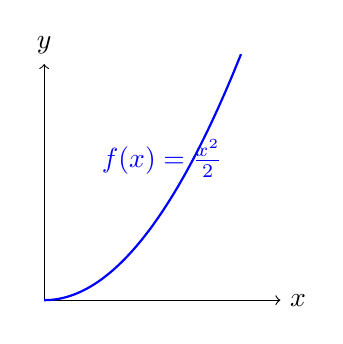
\begin{tikzpicture}
    \draw[->] (0,0) -- (3,0) node[right] {$x$};
    \draw[->] (0,0) -- (0,3) node[above] {$y$};
    \draw[domain=0:2.5,smooth,variable=\x,blue,thick]
        plot ({\x},{\x*\x/2});
    \node[blue] at (1.5,1.8) {$f(x) = \frac{x^2}{2}$};
\end{tikzpicture}

\subsection{Second Figure}

\tikzsetnextfilename{complex-diagram}
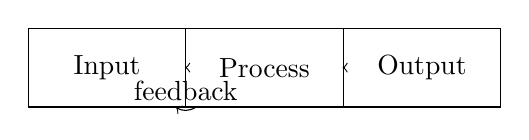
\begin{tikzpicture}[
    node distance=2cm,
    box/.style={rectangle, draw, minimum width=2cm, minimum height=1cm}
]
    \node[box] (a) {Input};
    \node[box, right of=a] (b) {Process};
    \node[box, right of=b] (c) {Output};

    \draw[->] (a) -- (b);
    \draw[->] (b) -- (c);
    \draw[->] (b) to[bend left] node[above] {feedback} (a);
\end{tikzpicture}

\subsection{Benefits}

\begin{itemize}
    \item Significantly faster recompilation (10x or more)
    \item Figures cached as individual PDFs
    \item Only modified figures are recompiled
    \item Reduces memory usage during compilation
\end{itemize}

\subsection{Security Note}

Externalization requires \texttt{-shell-escape}, which allows
LaTeX to execute system commands. \textbf{Only use with trusted
documents.} Modern TeX distributions use ``restricted shell escape''
for improved security.

\subsection{Makefile Integration}

\begin{verbatim}
# Makefile for TikZ externalization
all: document.pdf

document.pdf: document.tex
    latexmk -pdf -shell-escape document.tex

clean:
    latexmk -C
    rm -rf tikz-cache/

.PHONY: all clean
\end{verbatim}

\end{document}

% Notes:
% 1. Create tikz-cache/ directory before first compilation
% 2. Cached figures are named: fig-0.pdf, fig-1.pdf, etc.
% 3. Use \tikzsetnextfilename{} for reproducible names
% 4. See TikZ manual section "Externalization Library" for advanced options
